\section{Readout Electronic Design}
\label{sec:electronic_design}
The design of the readout electronics depends mainly on the directional radiation sensor (see sec. \ref{sec:radiation_sensor}) and the ASIC VATA466 (see \cite{Meier2016VATA466}) architecture and drive requirements.
The sensor needs a high voltage supply (see sec. \ref{sec:hv_supply}) to create a reverse bias, the ASIC (see sec. \ref{sec:vata466_baseboard}) is used to readout the sensor data.
The ASIC itself demands some stable supply voltages (see sec. \ref{sec:power_supplies}) and a bias current (see sec. \ref{sec:bias_current}).
To have access to the spectroscopic mode and for configuration purposes an ADC (Analog Digital Converter) is needed (see sec. \ref{sec:adc}).
Finally the power and data have to be interfaced with the rest of the cubesat (see sec. \ref{sec:interface_cubesat}).
The block diagram in fig. \ref{fig:electronic_block_diagram} shows the relationship between the different functional blocks of this electronic system.
\begin{figure}[H]
    \centering
    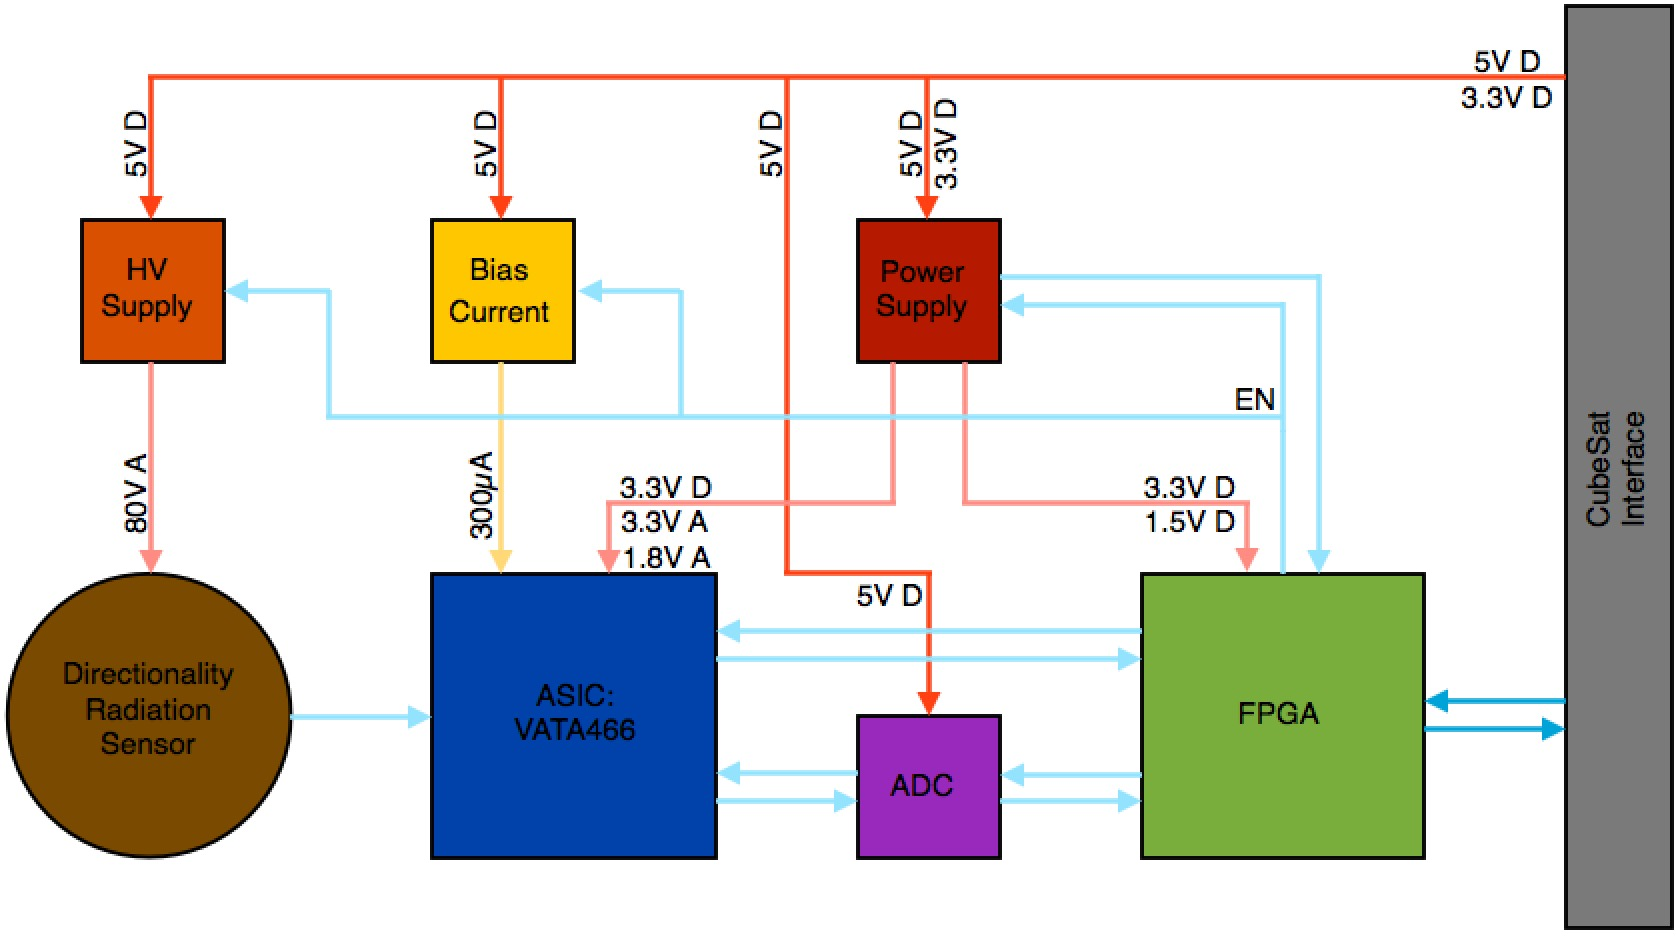
\includegraphics[width=1\textwidth]{electronic_block_diagram.jpg}
    \caption[Block Diagram Readout Electronics]{Block diagram of directional radiation sensor's readout electronics. \\(Power: Red Arrows, Data: Blue Arrows; D: Digital Voltage, A: Analog Voltage)}
    \label{fig:electronic_block_diagram}
\end{figure}

The design has to be optimized in terms of power consumption, size and radiation hardness. 
For the latter it was discussed with PSI that the final design could be tested for it's radiation resistance and therefore much cheaper and not officially radiation hardened components can be chosen.
Size and power considerations mainly have to be traded off against signal quality.

It is important to stay in the boundaries given by the data sheet of the ASIC to ensure a correct functioning of the instrument.

\subsection{VATA466 Baseboard}
\label{sec:vata466_baseboard}
The schematic ``VATA466\_Base\_Board.SchDoc'' (see app. \ref{sec:schematics}, p. 1/17) includes all the basic building blocks of the electronic design and therefore resembles largely to the block diagram and description in section \ref{sec:electronic_design}.
A data bus connects all the command and data lines between the different modules and the FPGA.
A power bus distributes the correct voltages to the specific systems.

\subsubsection{ASIC: VATA466}
\label{sec:asic}
In the schematic ``VATA466.SchDoc'' (see app. \ref{sec:schematics}, p. 2/17) the ASIC is divided into his functional sub parts.
Figure \ref{fig:signals_pads} shows a schematic representation of the ASIC's functions and pins.
\begin{figure}[H]
    \centering
    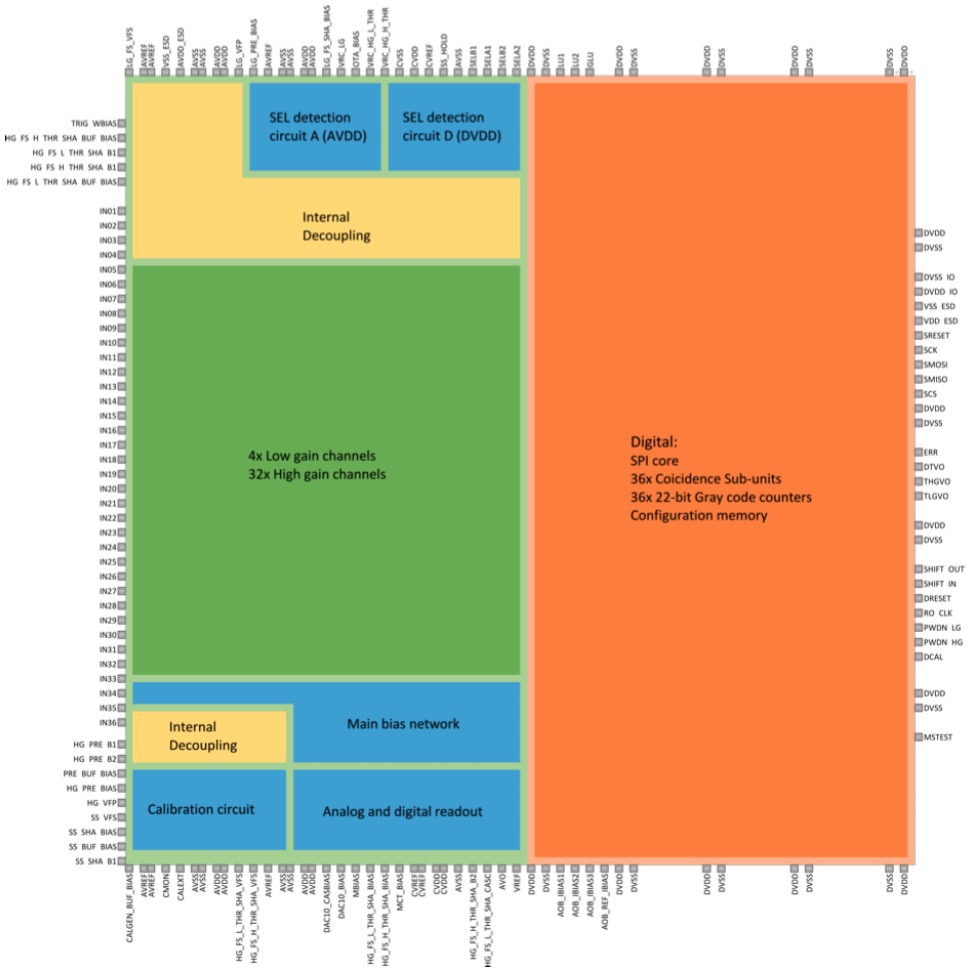
\includegraphics[width=\textwidth]{signals_pads_chip.jpg}
    \caption[Signals and Chip Pad Frame]{Schematic overview of sub parts and pins of the ASIC.\cite[p. 14, fig. 3]{Meier2016VATA466}}
    \label{fig:signals_pads}
\end{figure}

There are 36 charge sensitive pre-amplifiers (U19A), 4 of them have a low gain and 32 a high gain.
The DRS has 31 detector diodes and therefore uses 31 inputs of the high gain channels.

The ASIC also contains two power sub parts, an analogue one (U19B) and a digital one (U19C).
They differ in that the analogue input voltages have strict requirements and need to have low noise since they interact directly with the signals in the ASIC.
The digital input voltage is only used for the logic in the ASIC and is therefore less critical.
These inputs should be strictly isolated to avoid any degradation of the measurements.
The supply voltages will be discussed in more detail in section \ref{sec:power_supplies}.

The next sub unit of the ASIC holds all his bias and test-pads (U19D).
The bias network will be described in more detail in section \ref{sec:bias_current}.
The test-pads can be used to debug the ASIC and to directly readout some of it's internal signals.
The following table describes the pins purposes and gives recommendations for external decoupling:
\begin{table}[H]
	\centering
    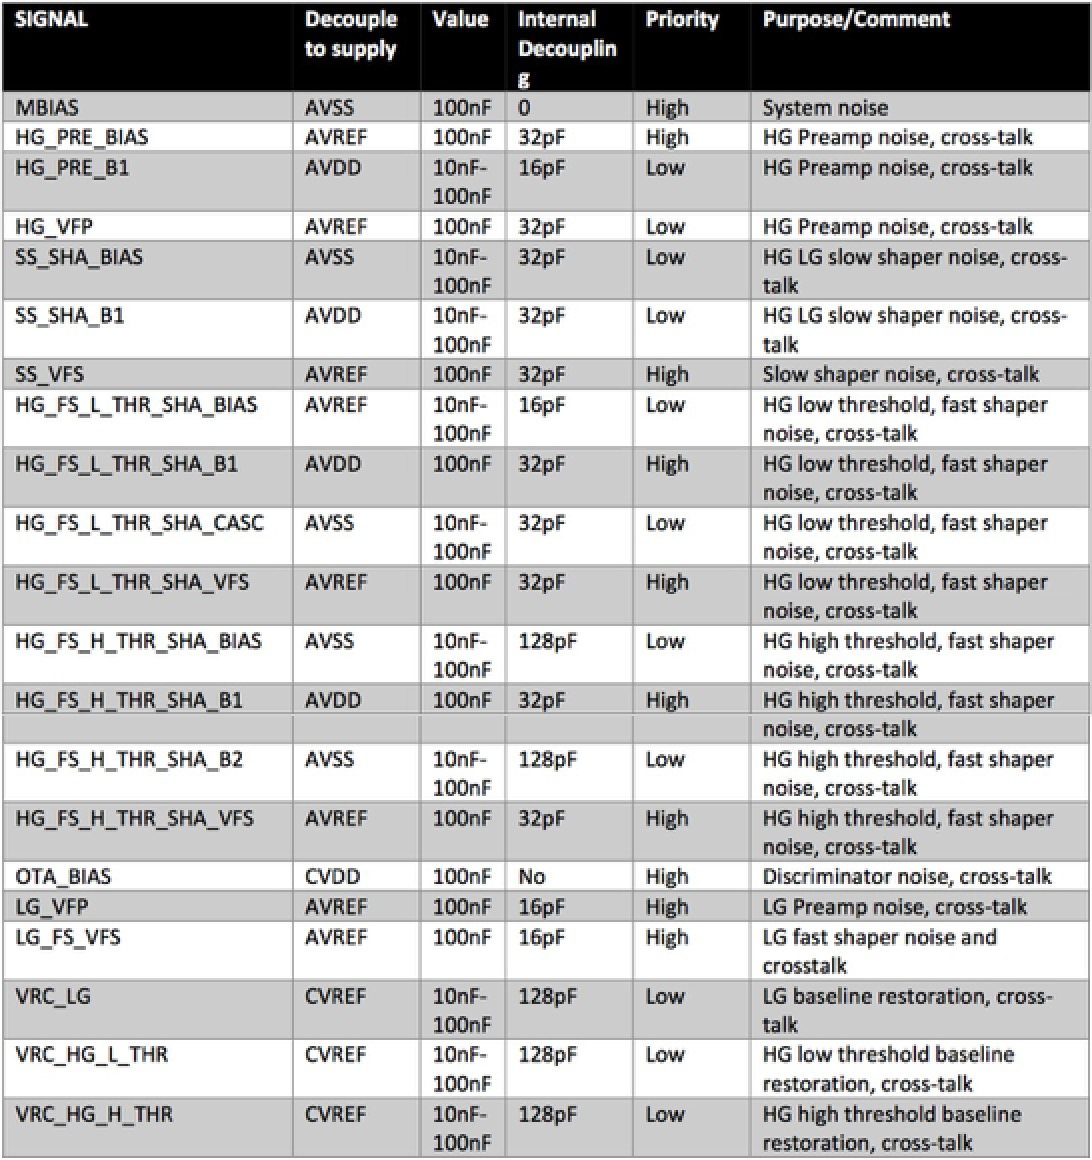
\includegraphics[width=0.8\textwidth]{test-pins.jpg}
    \caption[Test-pins Purpose and External Decoupling]{Purposes of the different test-pins and recommendations for external decoupling.\cite[p. 65-66, tab. 31]{Meier2016VATA466}}
	\label{tab:test-pads}
\end{table}

The last sub part of the ASIC regroups all pins used for the readout and commands (U19E).
It uses SPI (Serial Peripheral Interface) to read or write over the ASIC's registers and thereby enables the use of the counting mode.
A calibration sub unit can be used to test and calibrate the gain in the pre-amplifier, slow shapers and trigger the increment of a counter in a channel.
The power down block is used to power down the 4 low gain channels (1 to 4) and/or 16 high gain channels (21 to 36), channels 5 to 20 are always powered on.
A single analogue output is provided through the AVO pin, which allows the readout of the pulse heights from all channels via multiplexing (see sec. \ref{sec:adc}).
The multiplexer is controlled through the A\&D channel readout block and is therefore used to setup the spectroscopic mode of the ASIC.
The trigger out block is used to indicate the triggering of either a low-gain or high-gain channel or the digital multiplexer.
The last block enables the latch-up detection in the ASIC and will be further explained in the next section.\cite{Meier2016VATA466}

\subsubsection{Latch-up Detector}
\label{sec:latchup_detector}
There are two latch-up detection modules included in the ASIC.
They each have two inputs SELA and SELB and one output LU.
A global latch-up signal (GLU) is created through a logic OR between the two latch-up detector outputs.
The schematic ``Latch\_Up\_Power.SchDoc'' (see app. \ref{sec:schematics}, p. 3/17) represents an implementation of the recommended external circuit (see fig. \ref{fig:latch-up}).
\begin{figure}[H]
    \centering
    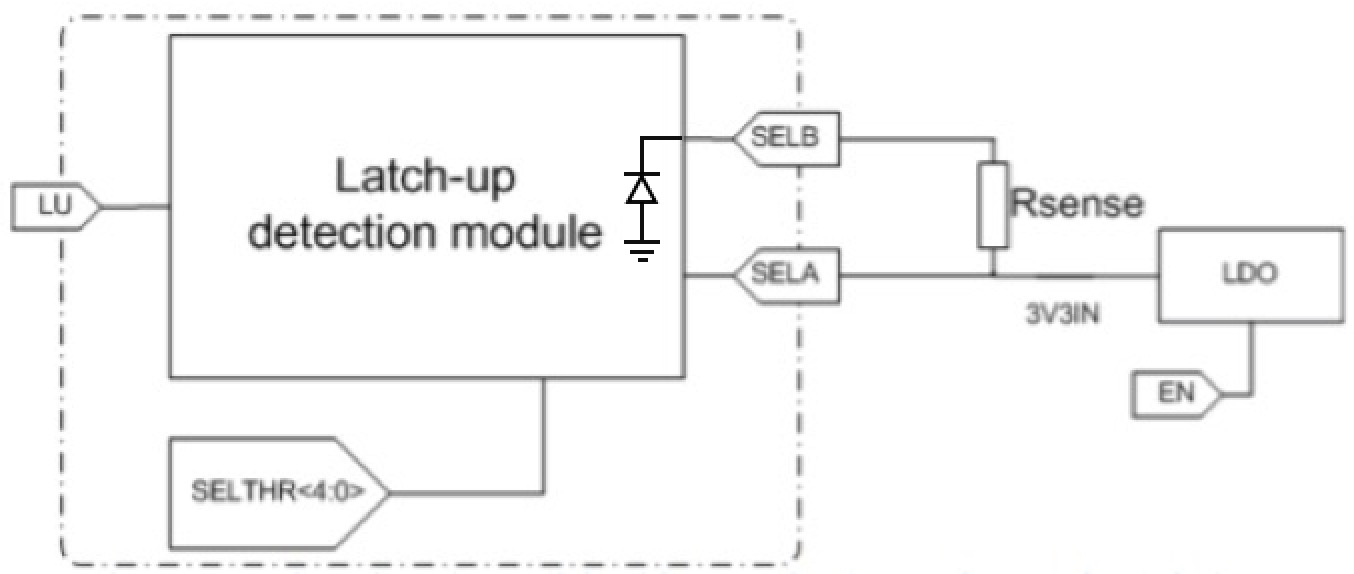
\includegraphics[width=0.6\textwidth]{latch-up.jpg}
    \caption[Latch-up Detection Module]{Reference design of an external latch-up detection circuit.\cite[p. 66, fig. 12]{Meier2016VATA466}}
    \label{fig:latch-up}
\end{figure}

The circuit consists of a LDO (U7 \& U8\footnote{LT1763}) which provide a constant 3.3V.
The detector can be seen as a simple diode.
As long as there is no SEL (Single-Event Latch-up), there will be no voltage drop over $R_{sense}$.
A SEL would make the diode conducting and there would be a voltage drop between the SELA and SELB pins.
This voltage is compared to the threshold value (SELTHR).
Being above it, the corresponding LU pin is set to high and therefore the GLU pin will go to high as well and indicate a latch-up.\cite[p. 66-68, fig. 12]{Meier2016VATA466}

\subsection{High Voltage Supply}
\label{sec:hv_supply}
A high voltage supply is needed to induce the reverse bias on the DRS's diodes.
Depending of their lifetime and sensitivity they should be biased with 40-60 V.\footnote{A bias of 80V could be imagined, which might make it possible to share a single high voltage supply between the DRS from PSI and the sensors from RUAG.} 

The circuit ``HV\_Power.SchDoc'' (see app. \ref{sec:schematics}, p. 4/17) uses an extra-small high voltage biasing supply (U9\footnote{0.1XS5-P0.1}).
A 5V input voltage is required to create a 0-100V output voltage with a maximum output current of 1mA.
To adjust the high voltage output, a 12 bit DAC (Digital Analog Converter) with reset to zero scale (U10\footnote{LTC2631}) was chosen.
The zero scale reset is important to prevent uncontrolled voltage spikes on power-on and therefore make the system initialization consistent and repeatable.
The DAC produces an output voltage of 0-2.5V which is proportional to the high voltage output of the supply of 0-100V.
A serial $I^2C$ interface is used to operate the DAC.

\subsection{Directional Sensor}
\label{sec:directionality Sensor}
As explained in section \ref{sec:radiation_sensor}, the DRS is composed of 31 sensing diodes, a large anode and guard rings.

In the ``Sensor\_Diodes.SchDoc'' schematic (see app. \ref{sec:schematics}, p. 13/17) a typical connection of the sensing diodes is shown.
A high voltage (40-80V) is applied on the cathode and the anode is connected to GND to apply the reverse bias.
When radiation passes through the depletion region a current is induced.
This current passes through a resistor, so that at the output a voltage can be read.
The trade-off for this resistor is done between the sensitivity and noise, a value of $2.2M\Omega$ was defined by PSI.

The schematic ``Shield\_Sensor.SchDoc'' (see app. \ref{sec:schematics}, p. 14/17) shows both, the concept of the large anode and a guard ring.
Both are split up in 4 equal sub-circuits.
This approach allows a symmetric distribution of the contacts around the circular detector, which in turn makes the protective effects more symmetric and therefore more effective. 

The large anode is basically connected with a resistor and capacitor.
The resistor will define current flow and the capacitor will collect the created charges to avoid noise from the area around the detector diodes.
The capacitors should be chosen as big as possible, so that a large number of charges can be buffered.
On the other hand this capacitor needs to be compatible with the large biasing voltage, which implies a larger footprint.
A trade off has to be done considering the footprint of the capacitor.

The guard rings are band-shaped reverse biased diodes.
They will define the outer edge of the depletion region of the large anode and the sensors.
This is implemented to avoid leakage currents from the outside of the detector.

\subsection{Supply Voltages}
\label{sec:power_supplies}
A collection of supply voltages needs to be provided to the ASIC as well as the FPGA.
The ASIC (see tab. \ref{tab:asic_supply}) has pretty strict requirements on it's analog voltages (see sec. \ref{sec:analog_supply}).
The FPGA (see tab. \ref{tab:fpga_supply}) on the other hand has less strict requirements and it is possible to share one of the voltages with the digital supply (see sec. \ref{sec:digital_supply}) of the ASIC.
\begin{table}[H]
	\centering
    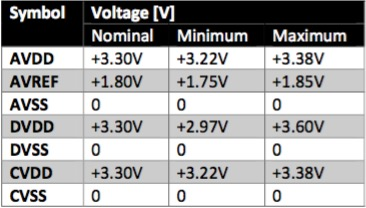
\includegraphics[width=0.4\textwidth]{asic_supply_voltages.jpg}
    \caption[ASIC Supply Voltages]{Requirements on the supply voltages for the ASIC.\cite[p. 82, tab. 44]{Meier2016VATA466}}
	\label{tab:asic_supply}
\end{table}
\begin{table}[H]
	\centering
    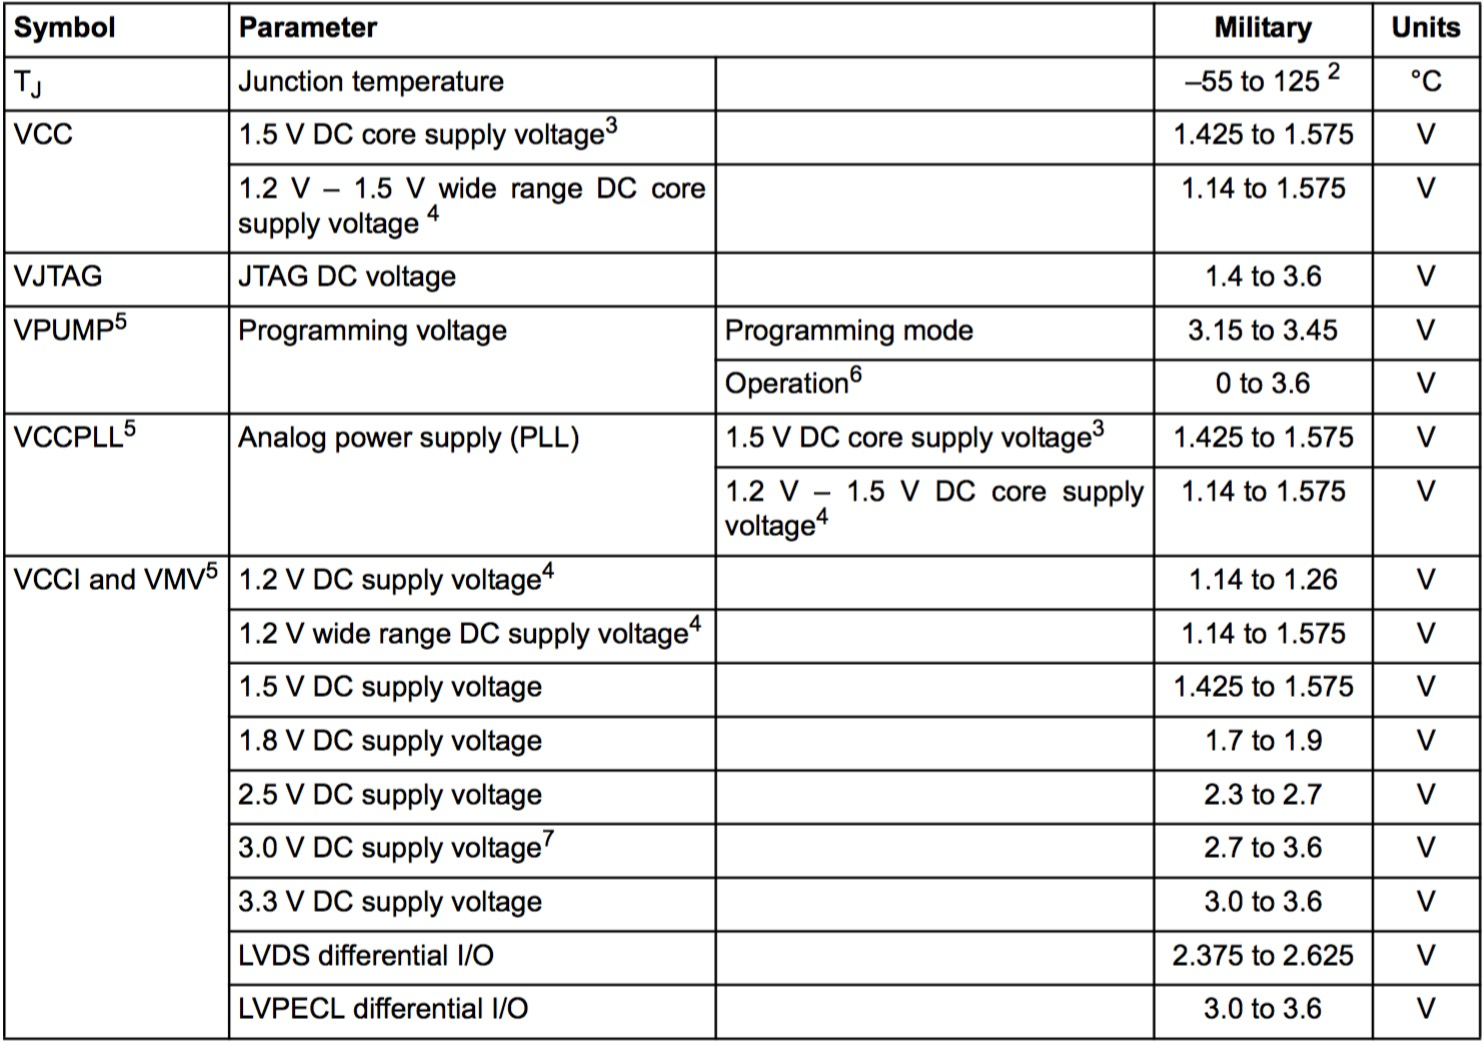
\includegraphics[width=0.65\textwidth]{fpga_supply_voltages.jpg}
    \caption[FPGA Supply Voltages]{Requirements on the supply voltages for the FPGA.\cite[p. 2-2, tab. 2-2]{microsemi2014military}}
	\label{tab:fpga_supply}
\end{table}

A trade-off had to be done between circuit area, power consumption and the amount of housekeeping data.
As can be seen in the ``BB\_Power.SchDoc'' (see app. \ref{sec:schematics}, p. 5/17), it was decided that there will be one point of current, voltage and temperature measurement (U16 \& U17\footnote{MAX9611}) in front of both the digital power block and the analog power block.

\subsubsection{Analog Supply Voltages}
\label{sec:analog_supply}
The analog supply voltage block is isolated from any logic noise and is represented in the schematic ``Analog\_Power.SchDoc'' (see app. \ref{sec:schematics}, p. 6/17).
The AVDD and CVDD share a common 3.3V power supply, as allowed by the data sheet.
A 1.8V power supply is used for AVREF.
There is also a shunt regulator which provides sink capability for the CVREF pin.

Both power supplies use a LDO (U1 \& U6\footnote{LT3042}) to create the required voltages from a 5V input.
They have very low noise ($0.8 \mu V_{RMS}$) and a programmable current limit, which can protect the ASIC in case of SELs.
The output voltage can be set by a resistor to GND at the SET pin using the formula $V_{SET} = I_{SET}\cdot R_{SET}$.
This results in a $33k\Omega$ resistor for the 3.3V supply and a $18k\Omega$ resistor for the 1.8V supply.
The current limit was set to 200 mA, using $I_{LIM} = \frac{125mA}{R_{LIM}}$ we find a required resistor of $620\Omega$.

The power supplies also use a digital isolator (U3 \& U5\footnote{ADUM1100}) to drive enable or disable the voltage, without inducing noise into the output.
A digital coupling was chosen over an optical coupling because it is more resistant to radiation and harsh environments.

A shunt regulator (U7\footnote{TLHV431}) is used to provide sink capability to the CVREF pin while keeping it at around 1.8V.
Schematic ``CVREF\_Sink.SchDoc'' (see app. \ref{sec:schematics}, p. 9/17) shows it's design.
Using the formula $V_O = (1+\frac{6.2k\Omega}{15k\Omega})V_{REF}$ results in an output voltage of 1.75V.

\subsubsection{Digital Supply Voltages}
\label{sec:digital_supply}
The digital supply voltages in schematic ``Digital\_Power.SchDoc'' (see app. \ref{sec:schematics}, p. 10/17) provide systems with power which are not critically affected by noise coming from any logic components.
Both the ASIC and the FPGA need a supply voltage of 3.3V, which is directly sourced from the satellites power bus, filtered and then shared between them.
The 1.5V for the FPGA is created by using a small LDO (U4\footnote{LT1963}).


\subsection{Bias Current}
\label{sec:bias_current}
In order for the ASIC to generate all internal bias currents and bias voltages, one external current source called MBIAS is needed.
The maximum operation voltage of the device is given to be 3.6V, therefore the current source shall not exceed this voltage.
Further requirements of the current source are described in the following table:\cite[p. 64-65]{Meier2016VATA466}
\begin{table}[H]
	\centering
    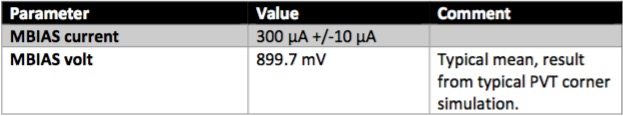
\includegraphics[width=0.6\textwidth]{mbias.jpg}
    \caption[MBIAS Parameters]{Requirements on MBIAS current source.\cite[p. 65, tab. 30]{Meier2016VATA466}}
	\label{tab:mbias}
\end{table}

\subsubsection{Current Source Variations}
\label{sec:current_source}
A \textbf{Zener diode current source} (see fig. \ref{fig:zener_current_source}) is one of the most simple forms.
It uses the fact that a reverse biased Zener diode has a constant voltage drop ($V_Z$) across it, irrespective of the current ($I_Z$) flowing through it.
The resistor R1 is used to induce a current above the holding current in the Zener diode.
The voltage over R2 is given by $V_{R2} = V_Z - V_{BE}$, where $V_{BE}$ is the base-emitter voltage of Q1.
This gives us the current in the load, which is the same as the emitter current of Q1 and the current in R2 ($I_{R2}$) and is given by $I_{Load} = I_E = I_{R2} = \frac{V_{R2}}{R2} = \frac{V_Z-V_{BE}}{R2}$.
\begin{figure}[H]
    \centering
    \includegraphics[width=0.3\textwidth]{zener_current_source.png}
    \caption[Zener Current Source]{A basic Zener diode current source.\cite{wikipedia2016current}}
    \label{fig:zener_current_source}
\end{figure}

An \textbf{op-amp current source} (see fig. \ref{fig:op-amp_current_source}) can be used to improve the circuit explained above.
The principle is the same as above, with the difference that a feedback loop is created by adding an op-amp.
It actively keeps up the constant voltage ($V_Z$), defined by the Zener diode, over the sense resistor ($R_{sense}$).
Therefore the current through the load is constant and defined as $I_{Load} = I_{sense} = \frac{V_Z}{R_{sense}}$.
\begin{figure}[H]
    \centering
    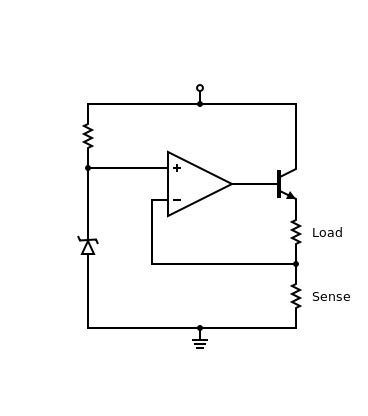
\includegraphics[width=0.3\textwidth]{op-amp_current_source.png}
    \caption[Op-amp Current Source]{Op-amp current source.\cite{wikipedia2016current}}
    \label{fig:op-amp_current_source}
\end{figure}

\subsubsection{MBIAS Design}
\label{sec:mbias_design}
The schematic ``MBIAS.SchDoc'' (see app. \ref{sec:schematics}, p. 11/17) represents a more complex approach based on a basic op-amp current source (see fig. \ref{fig:mbias_op-amp_source}).
The Zener diode (D33\footnote{LT1634}) with a reverse bias of $V_Z = 1.25V$ is kept above the holding current by the current $I_Z = I_{R45} = \frac{V_D-V_Z}{R45} = \frac{1.5-1.25}{24k\Omega}$ created in R45, with $V_D = 1.5V$ being the drive voltage.
The op-amp (U12B\footnote{LTC6078}) uses $V_Z$ to keep a constant voltage drop of 0.25V over the two resistors R2 and R3, they are connected in series and together fulfill the function of $R_{sense}$ from above.
The transistor Q1 drives the current $I_{MBIAS} = \frac{0.25V}{R2+R3} = \frac{0.25V}{825\Omega+8.2\Omega}$ to the MBIAS pin.
The maximal output voltage is limited to $V_{max} = V_Z = 1.25V$.
\begin{figure}[H]
    \centering
    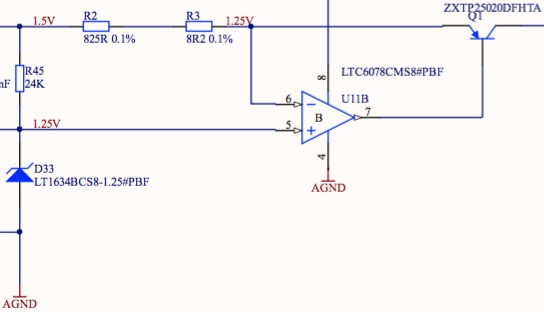
\includegraphics[width=0.55\textwidth]{mbias_op-amp_source.jpg}
    \caption[MBIAS Op-amp Current Source]{MBIAS op-amp current source.}
    \label{fig:mbias_op-amp_source}
\end{figure}

Another advantage of this design is it's drive voltage that is internally created by the second half of the circuit (see fig. \ref{fig:mbias_power_supply}) and is therefore independent of a possibly unstable external power supply.
The same Zener diode as above (D33), with a reverse bias of $V_Z = 1.25V$, is used as a reference for the drive voltage $V_D = 1.5V$.
The resistors R34 and R35 define the gain of the op-amp (U12A) as $g = \frac{R2}{R1}+1 = 1.2$, which results in a drive voltage of $V_D = g\cdot V_Z = 1.5V$.
For this circuit to work the differential input voltage has to be positive, which is not necessarily the case during power-up.
Therefore we use C21 to pull the positive entry of the op-amp above the negative one.
\begin{figure}[H]
    \centering
    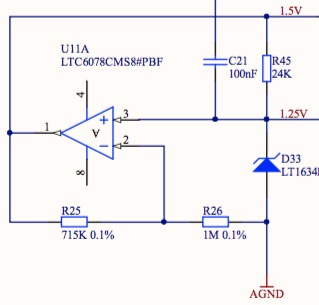
\includegraphics[width=0.4\textwidth]{mbias_power_supply.jpg}
    \caption[MBIAS Voltage Generation]{Internal and passive Voltage generation for MBIAS.}
    \label{fig:mbias_power_supply}
\end{figure}

The remaining part of the circuit is a digital coupler (U12\footnote{ADUM1100}) that controls a FET (Field Effect Transistor) (Q2\footnote{BSS138}) which switches the current source on or off.

\subsection{Analog Digital Converter}
\label{sec:adc}
Schematic ``ADC.SchDoc'' (see app. \ref{sec:schematics}, p. 12/17) shows an ADC design that can both be used to readout AVO in spectroscopic mode and to monitor the calibration voltage on CMON.
It uses a 12 bit differential input ADC (U15\footnote{AD7452}) with 555 ksps (Kilosamples per Second).
A high accuracy voltage reference (U14\footnote{ADR4533}) is used to provide $V_{REF}$ to the ADC.
One of the differential inputs can be connected to AVO or CMON respectively.
The second input shall be connected to GND in close proximity to the respective measurement pin, so that the resistance of the lines don't influence the measurement.
The ADC is connected to the FPGA using SPI.

\subsection{FPGA}
\label{sec:FPGA}
The ``FPGA.SchDoc'' (see app. \ref{sec:schematics}, p. 16/17) schematic defines a basic layout of an FPGA\footnote{A3P1000-FG144M} drive circuit.
J1\footnote{Connector: 3020-10-0300-00} provides a standard interface for programming the FPGA's logic.
The IO pins of the IO banks are not yet defined. 
That is mainly due to one reason:
There are about 22 digital CMOS\_3V3 I/O pins that directly interface with the ASIC. 
In this project, only the CMA digital hardware was developed and documented, a maximum of 6 pins is allocated for this part of the readout. 
For a prototype board, the I/O assignment is insignificant. 
It is recommended to connect the FPGA and ASIC pins by other means then conducting tracks for the purpose of oscilloscope tests. 
The pins on the FPGA can be re-assigned by small changes in the program code.

\subsection{Interface CubeSat}
\label{sec:interface_cubesat}
The interface to the cubesat is not defined in much detail yet.
The proposed readout electronics assume a power bus that provides 3.3V and 5V.
As of now there is no data bus defined.
The size of the FPGA allows for a quick implementation and adaption to most common variants like the CAN bus.
A programming interface is provided in the FPGA schematics.
